\documentclass{standalone}
\usepackage[latin1]{inputenc}
\usepackage{amsmath,amssymb,mathtools,mathrsfs}
\usepackage[T1]{fontenc}
\usepackage{tikz}
%\usepackage{amsthm}
%\usepackage[all]{xy}
%\usepackage{enumerate}
%\usepackage[hidelinks]{hyperref}

%\addtolength{\oddsidemargin}{-3cm}
%\addtolength{\evensidemargin}{-1cm}
%\addtolength{\textwidth}{2cm}
%\addtolength{\topmargin}{-2cm}
%\addtolength{\textheight}{2cm}


\date{\today}
\begin{document}
%\author{Florent Martin}

\title{}
%\maketitle
%\tableofcontents

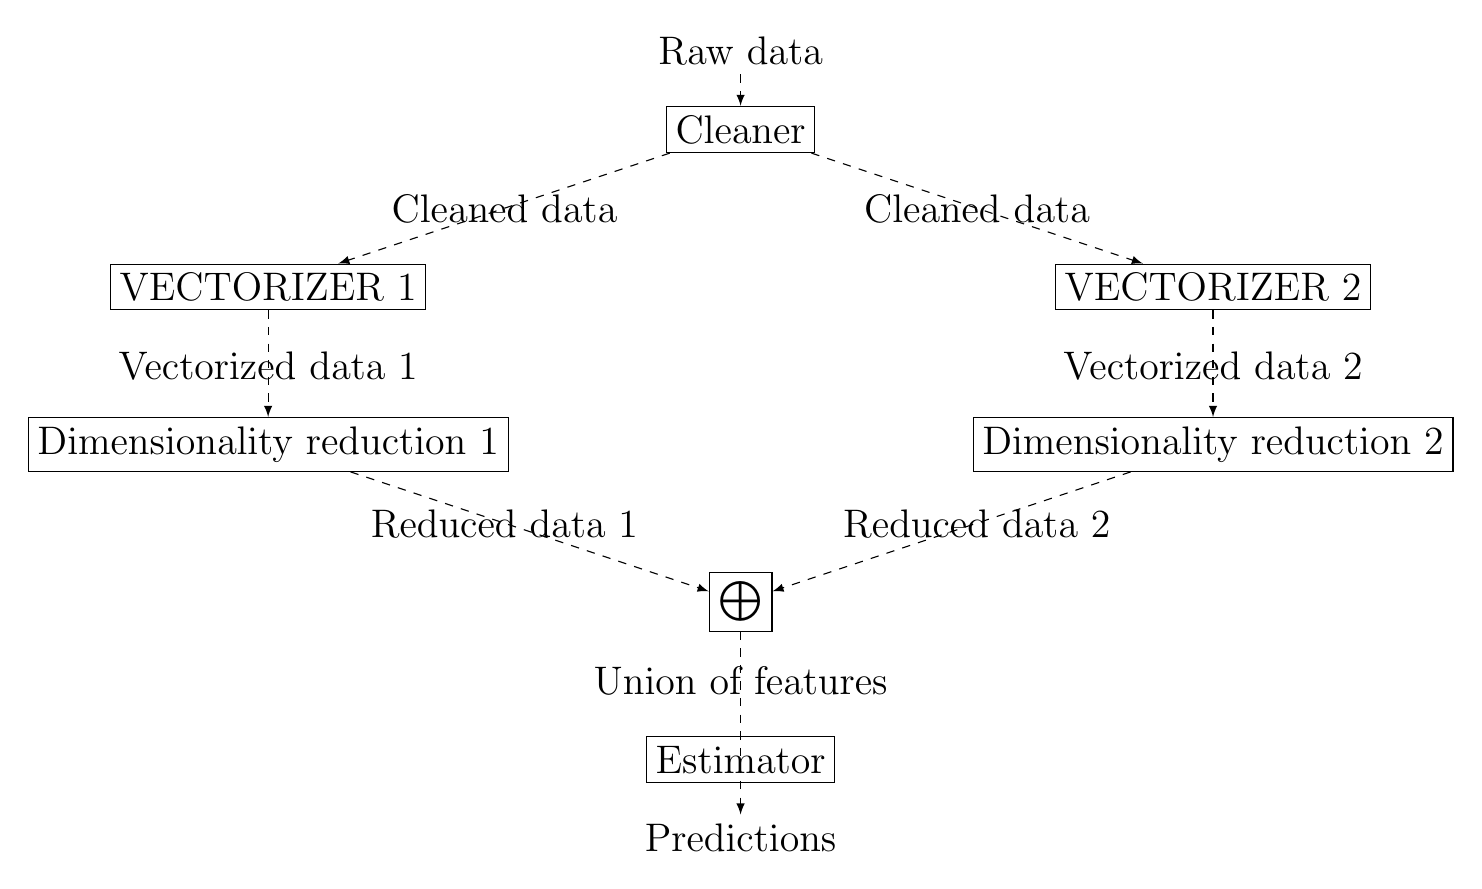
\begin{tikzpicture}

\tikzstyle{every node}=[font=\Large]
%or \LARGE, \huge \HUGE


\pgfmathsetmacro\x{0}
\pgfmathsetmacro\y{0}

\node (raw) at (\x, \y) {Raw data};

\pgfmathsetmacro\y{\y-1}
\node[draw] (cleaner) at (\x, \y) {Cleaner};

\draw[->,>=latex,dashed] (raw) -- (cleaner);

\pgfmathsetmacro\y{\y-1}
\node (cleanded1) at (\x-3, \y) {Cleaned data};
\node (cleanded2) at (\x+3, \y) {Cleaned data};


\pgfmathsetmacro\y{\y-1}
\node[draw] (vectorizer1) at (\x-6,\y) {VECTORIZER 1};
\node[draw] (vectorizer2) at (\x+6,\y) {VECTORIZER 2};

\draw[->,>=latex,dashed] (cleaner) -- (vectorizer1);
\draw[->,>=latex,dashed] (cleaner) -- (vectorizer2);

\pgfmathsetmacro\y{\y-1}
\node (vecotorized1) at (\x-6, \y) {Vectorized data 1};
\node (vecotorized2) at (\x+6, \y) {Vectorized data 2};


\pgfmathsetmacro\y{\y-1}
\node[draw] (reducer1) at (\x-6,\y) {Dimensionality reduction 1};
\node[draw] (reducer2) at (\x+6,\y) {Dimensionality reduction 2};

\draw[->,>=latex,dashed] (vectorizer1) -- (reducer1);
\draw[->,>=latex,dashed] (vectorizer2) -- (reducer2);

\pgfmathsetmacro\y{\y-1}
\node (reduced_vecotorized1) at (\x-3, \y) {Reduced  data 1};
\node (reduced_vecotorized2) at (\x+3, \y) {Reduced  data 2};

\pgfmathsetmacro\y{\y-1}
\node[draw] (union) at (\x,\y) {$\bigoplus$};

\draw[->,>=latex,dashed] (reducer1) -- (union);
\draw[->,>=latex,dashed] (reducer2) -- (union);

\pgfmathsetmacro\y{\y-1}
\node (unioned) at (\x,\y) {Union of features};

\pgfmathsetmacro\y{\y-1}
\node[draw] (estimator) at (\x,\y) {Estimator};

\pgfmathsetmacro\y{\y-1}
\node (predictions) at (\x,\y) {Predictions};

\draw[->, >=latex, dashed] (union) -- (predictions); 

\end{tikzpicture}

%\bibliographystyle{plain}
%\bibliography{../../Articles/bibli}

\end{document}
